\chapter{Arquitetura}
\begin{figure}[H]
	\centering
		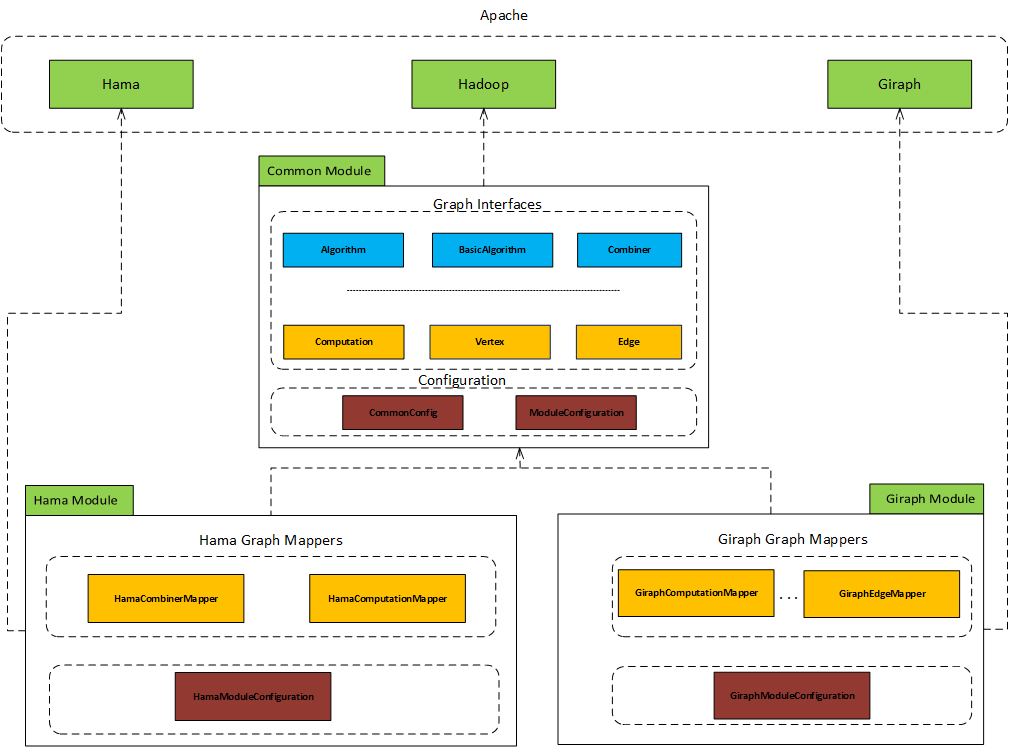
\includegraphics[width=\linewidth]{arquitetura}
	\caption{Em azul estão as interfaces e classes que devem ser 
	implementadas por um programador que esteja interessado em implementar 
um algoritmo no módulo comum. As outras cores representam interfaces e classes 
que devem ser implementadas para criar-se um novo módulo sobre o módulo comum.}
	\label{fig:arquitetura}
\end{figure}

Para que se torne possível a utilização das interfaces disponibilizadas pelo 
módulo comum existe a necessidade de realizar um conjunto de configurações. 
Devido a essa necessidade e para que essas 
configurações sejam feitas de forma independente da plataforma,
criou-se a interface \texttt{ModuleConfig} que será registada na classe \texttt{CommonConfig}.
Os módulos respetivos as plataformas que estão a mapear para o módulo comum necessitam implementar 
\texttt{ModuleConfig} e realizar as configurações necessárias para a respetiva 
plataforma. Esta implementação implica para que se use o módulo comum se proceda 
ao uso do \texttt{CommonConfig}.

O módulo comum foi construído de modo a que se possa fazer proveito das 
interfaces programáveis disponibilizas pelas plataformas Apache Giraph e Apache 
Hama. Usando o módulo comum é possível usar tipos de mensagens e tipos de valor 
para vértices diferentes, mesmo usando a plataforma Apache Hama onde isto não é 
possível. Igualmente, no Hama o tipo usado nos agregadores deve ser mesmo que o tipo
de valor dos vértices mas usando o módulo comum esta restrição é inexistente.

Contudo, nem todas as funcionalidades são disponibilizadas pelo módulo comum.
O \texttt{MasterCompute} não é disponibilizado devido a falta da sua implementação no Hama e dificuldade
de implementar-lo sem alterar diretamente o código da plataforma.
O \textit{input/output} é diferente nas 
duas plataformas daí que não exista nenhuma abstração no módulo comum.

Assim, é de seguida apresentado um exemplo de uso da plataforma.

\begin{verbatim}
		GiraphConfiguration conf = new GiraphConfiguration();

		// Configurações exclusivas à plataforma escolhida, como Input/Output, 
		// podem ser realizadas aqui
		
		//Para mudar a plataforma a ser usada bastaria mudar o ModuleConfiguration usado
		GiraphModuleConfiguration giraphConfig = new GiraphModuleConfiguration(conf);
		
		CommonConfig commonConfig = new CommonConfig(giraphConfig);
		
		// Configurações relacionadas com o algoritmo a correr
		commonConfig.setAlgorithmClass(ExampleAlgorithm.class);
		
		commonConfig.setCombinerClass(IntSumCombiner.class);
		
		commonConfig.registerAggregator("SumAgg", LongSumAggregator.class);
		commonConfig.registerAggregator("OrAgg", BooleanOrAggregator.class);
		
		// Precisa sempre de ser chamado para configurações finais
		commonConfig.preparePlatformConfig();
\end{verbatim}
